\documentclass[DIV=calc, paper=a4, fontsize=11pt]{scrartcl}


\usepackage{makeidx}
\usepackage{graphicx}
\usepackage{flushend}

\usepackage{lmodern}
\usepackage[left=1.5cm,right=1.5cm,top=2.5cm,bottom=2cm]{geometry}
\usepackage{float}		
\bibliographystyle{plain} 
\pagestyle{plain} 
\pagenumbering{arabic}
\usepackage{fancyhdr} 	


\usepackage[T1]{fontenc}
\usepackage[utf8]{inputenc}
\usepackage[spanish]{babel}
\usepackage{hyperref}
\usepackage{graphicx}
\usepackage{siunitx}

\usepackage{lipsum}
\usepackage[protrusion=true,expansion=true]{microtype}
\usepackage{amsmath,amsfonts,amsthm}
\usepackage[svgnames]{xcolor}
\usepackage[svgnames]{xcolor}
\usepackage{booktabs}
\usepackage{fix-cm}
\usepackage{multicol}
\newenvironment{Figura}
  {\par\medskip\noindent\minipage{\linewidth}}
  {\endminipage\par\medskip}

\usepackage{sectsty}
\allsectionsfont{\usefont{OT1}{phv}{b}{n}}

\usepackage{fancyhdr}
\pagestyle{fancy}
\usepackage{lastpage}

\lhead{}
\chead{}
\rhead{}

\lfoot{}
\cfoot{}
\rfoot{\footnotesize Page \thepage\ of \pageref{LastPage}}

\renewcommand{\headrulewidth}{0.0pt}
\renewcommand{\footrulewidth}{0.4pt}

\usepackage{lettrine}
\newcommand{\initial}[1]{\lettrine[lines=3,lhang=0.3,nindent=0em]{
\color{DarkGoldenrod}{\textsf{#1}}}{}}

\usepackage{titling}

\newcommand{\HorRule}{\color{DarkGoldenrod} \rule{\linewidth}{1pt}}

\pretitle{\vspace{-120pt} \begin{flushleft} \HorRule \fontsize{22}{35} \usefont{OT1}{phv}{b}{n} \color{DarkRed} \selectfont}

\title{Intensidad y decaimiento del sonido\\ %Aquí va el nombre de la práctica 
Práctica 2} %Numero de la práctica 

\posttitle{\par\end{flushleft}\vskip 0.5em}

\preauthor{\begin{flushleft}\large \lineskip 0.5em \usefont{OT1}{phv}{b}{sl} \color{DarkRed}}

\author{Misael Iván Macías Márquez\\
misaelmacias@ciencias.unam.mx}

\postauthor{\footnotesize \usefont{OT1}{phv}{m}{sl} \color{Black}

\vspace*{0.1cm} Facultad de Ciencias, UNAM

\par\end{flushleft}\HorRule}

\date{Domingo 13 de Marzo de 2022\\Semestre 2022-1}


\begin{document}

\maketitle


\begin{abstract}
\textbf{Resumen:} Se midieron las intensidades generadas por una computadora para un rango especifico de frecuencias con ayuda de un sonómetro y una cámara de teléfono, se observo al graficar distancia vs nivel de sonido vs frecuencia que para cada frecuencia se tiene aproximadamente la misma tendencia solo que al ir aumentando esta tendencia se desplaza hacia arriba en la intensidad hasta un punto máximo donde parece detenerse, también se observo que para frecuencias aproximadamente por debajo de los $400Hz$ la pendiente ajustada por mínimos cuadrados corresponde con el valor esperado  pero para frecuencias altas el error ya es considerable.


\end{abstract}

\begin{multicols}{2}




\section*{Introducción}

Las ondas sonoras son ondas mecánicas longitudinales que viajan a través de solidos, líquidos y gases. Estas ondas mecánicas se pueden considerar como cambios de presión en el medio sobre el que se encuentre inmerso o desplazamientos del mismo[2].

El ser humano es capaz de escuchar estas ondas mientras se encuentren en un rango de frecuencias de 20 a 20,000 Hertz (Hz), las frecuencias sobre este rango se llaman ultrasónicas y las que se encuentran debajo son infrasónicas[2].



Una magnitud util al comparar sonidos es la intensidad ($I$) que es:

\begin{equation}
    I = \frac{\hat{P}}{A}
\end{equation}

\noindent donde $\hat{P}$ es la potencia promedio y $A$ es el área por la que se propaga la onda sonora, entonces al suponer que estas ondas longitudinales se propagan formando una esfera de radio $r$, la intensidad ($I$) descrita por la misma queda como[2]:

\begin{equation}
    I \frac{\hat{P}}{4 \pi r^2}
\end{equation}

Dado que el oído humano es muy sensible, se utiliza una escala logarítmica para describir el nivel de sonido (SL) de la siguiente forma:

\begin{equation}
    SL = 10 \log_{10}{\frac{I}{I_0}}
\end{equation}

\noindent donde $I_0$ es el valor dado por la mínima audición humana ($\num{1e-12}W/m^2$), las unidades de $SL$ se conocen como decibelios ($dB$)[2].

Ahora sustituyendo la ecuación (2) en la (3) :

\begin{equation*}
    SL = 10 \log_{10}{\frac{\hat{P}}{4 \pi r^2 I_0}}
\end{equation*}

\noindent que por propiedades de los logaritmos es equivalente a:

\begin{equation*}
    SL = 10 \frac{\ln{\frac{\hat{P}}{4 \pi r^2 I_0}}}{\ln{10}}
\end{equation*}

\begin{equation*}
    \frac{\ln{10}\cdot SL}{10} = \ln{r^{-2}}+ \ln{\frac{\hat{P}}{4 \pi I_0}}
\end{equation*}

\begin{equation}
    \frac{\ln{10}\cdot SL}{10} =-2 \ln{r}+ \ln{\frac{\hat{P}}{4 \pi I_0}}
\end{equation}










\section*{Desarrollo experimental}

Con ayuda de una cinta métrica y un objeto medianamente pesado para mantener la cinta métrica recta se marcaron 11 distancias $r$ para cada 50 cm usando tapas de refresco en cada punto, sobre el primer punto se colocó la computadora con el generador de frecuencias y el volumen al máximo de tal forma que la bocina de la misma quedara lo mas centrada posible con la primera marca (tapita). También se optó por cortar varios papelitos que señalaran cada frecuencia usada y distancia para tener un mejor control de los resultados.

\begin{Figura}
\centering
    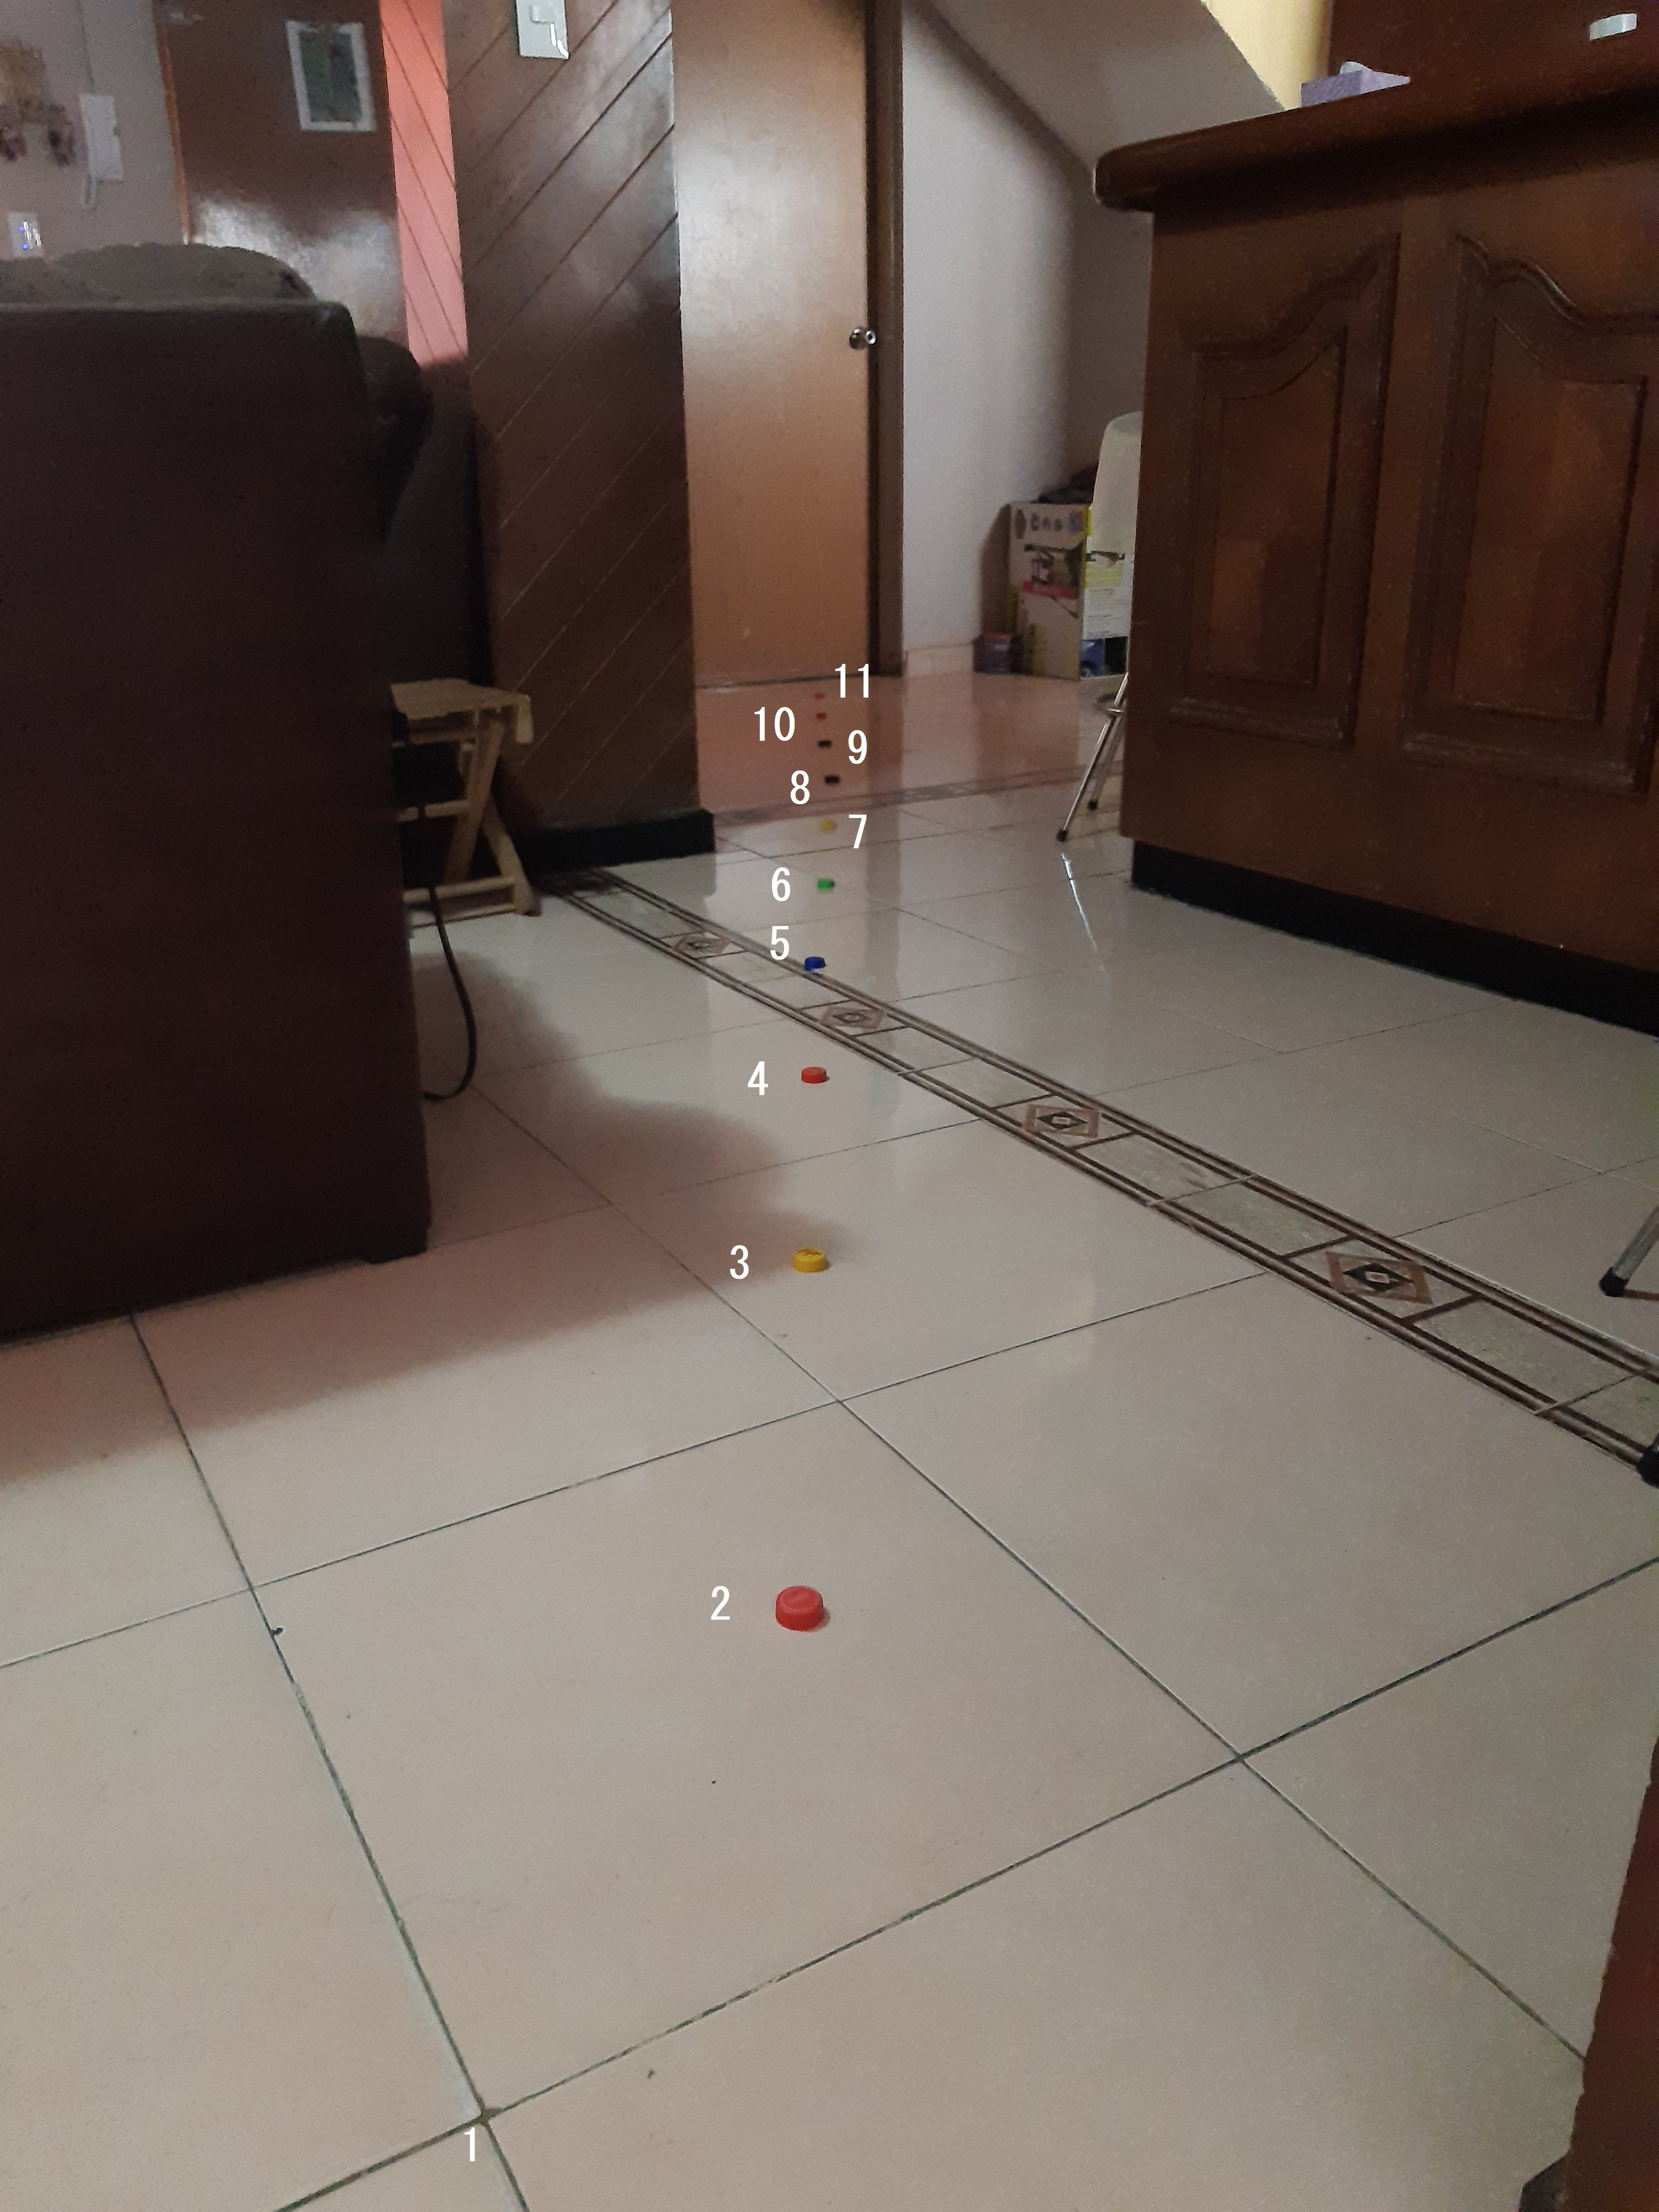
\includegraphics[width=0.8\textwidth]{20220226_145231.jpg}
    \captionof{figure}{Arreglo experimental: 1-11 tapas para marcar cada 50 cm, 1 computadora con el generador de frecuencias}
    \label{fig}
\end{Figura}

\begin{Figura}
\centering
    \includegraphics[width=0.8\textwidth]{20220226_150508.jpg}
    \captionof{figure}{Arreglo experimental desde otra perspectiva (lamento que esté al revés no logré corregir eso)}
    \label{fig}
\end{Figura}

Con el arreglo experimental ya listo, se utilizó un teléfono con un sonómetro para medir el nivel de sonido $SL$ de cada punto y otro con una cámara para registrar 30 segundos de intensidades medidas (para frecuencias altas se cortó el tiempo a 15 segundos debido a que lastimaban los oídos) las frecuencias utilizadas en el experimento fueron 10 separadas por $100Hz$, de $100 Hz$ a $1000 Hz$. 



\section*{Resultados y Análisis}

Lamentablemente al tener tanta variación en el tiempo grabado, se complicó bastante el tomar los promedios de cada video por lo que mejor se tomó un solo nivel de sonido de forma aleatoria como representativa de toda la muestra.

\begin{Figura}
\centering
    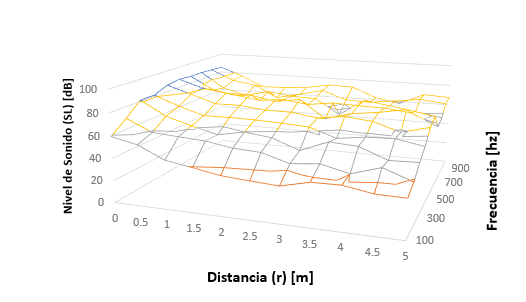
\includegraphics[width=1\textwidth]{grafica sonido 1.PNG}
    \captionof{figure}{Gráfica superficie de nivel de sonido ($SL$) vs distancia ($r$) vs frecuencia}
    \label{fig}
\end{Figura}

\begin{Figura}
\centering
    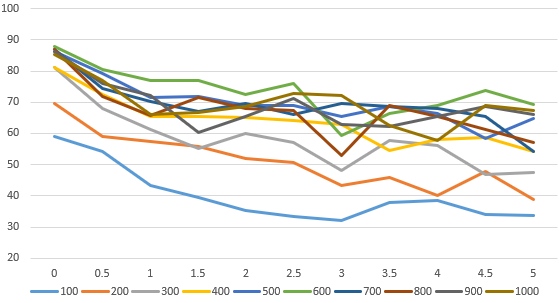
\includegraphics[width=1\textwidth]{grafica sonido 2.PNG}
    \captionof{figure}{Gráfica de cortes de superficie de nivel de sonido ($SL$) vs distancia ($r$) para cada frecuencia}
    \label{fig}
\end{Figura}



Usando la ecuación 4 se pueden transformar las mediciones obtenidas (ver apéndice) para tener una expresión linealizada donde $y = \frac{\ln{10} \cdot SL}{10}$, $m=-2$, $x= \ln{r}$ y $b= \ln{\frac{\hat{P}}{4\pi I_0}}$; así se obtiene la potencia de decaimiento ajustando la pendiente con el método de mínimos cuadrados.

Ahora veamos la propagación de incertidumbres de $y$ y $x$ en las figuras 5-14

\begin{equation*}
    \delta y = \sqrt{\left(\frac{\partial y}{\partial SL}\right)^2 \delta SL^2 } = \frac{\ln{10} \cdot \delta SL}{10}
\end{equation*}

y tambien

\begin{equation*}
    \delta x = \sqrt{\left(\frac{\partial x}{\partial r}\right)^2 \delta r^2} = \frac{\delta r}{r}
\end{equation*}



\begin{Figura}
\centering
    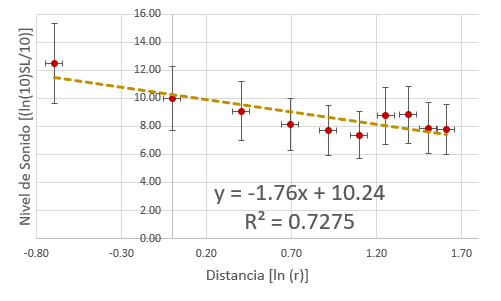
\includegraphics[width=1\textwidth]{grafica 100 Hz.PNG}
    \captionof{figure}{Gráfica del nivel de sonido vs la distancia para la frecuencia de $(100 \pm 1) Hz$}
    \label{fig}
\end{Figura}

\begin{Figura}
\centering
    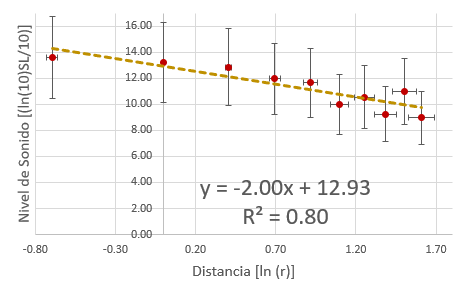
\includegraphics[width=1\textwidth]{grafica 200 Hz.PNG}
    \captionof{figure}{Gráfica del nivel de sonido vs la distancia para la frecuencia de $(200 \pm 1) Hz$}
    \label{fig}
\end{Figura}

\begin{Figura}
\centering
    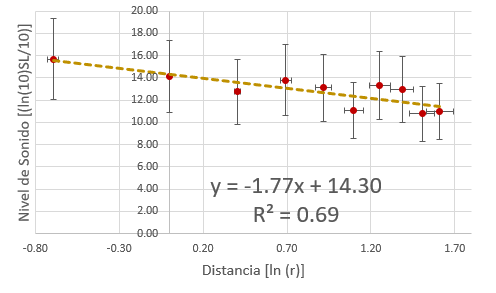
\includegraphics[width=1\textwidth]{grafica 300 Hz.PNG}
    \captionof{figure}{Gráfica del nivel de sonido vs la distancia para la frecuencia de $(300 \pm 1) Hz$}
    \label{fig}
\end{Figura}


\begin{Figura}
\centering
    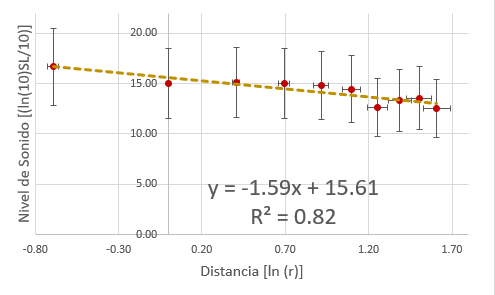
\includegraphics[width=1\textwidth]{grafica 400 Hz.PNG}
    \captionof{figure}{Gráfica del nivel de sonido vs la distancia para la frecuencia de $(400 \pm 1) Hz$}
    \label{fig}
\end{Figura}


\begin{Figura}
\centering
    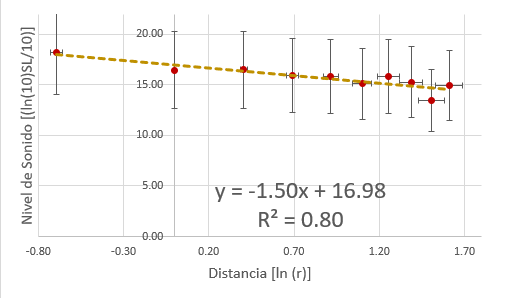
\includegraphics[width=1\textwidth]{grafica 500 Hz.PNG}
    \captionof{figure}{Gráfica del nivel de sonido vs la distancia para la frecuencia de $(500 \pm 1) Hz$}
    \label{fig}
\end{Figura}


\begin{Figura}
\centering
    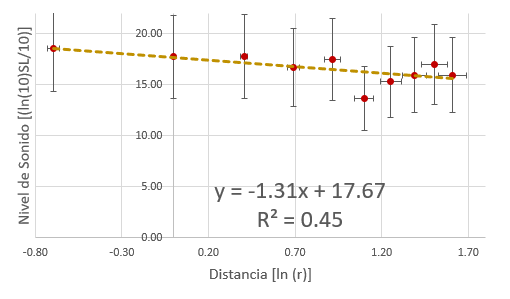
\includegraphics[width=1\textwidth]{grafica 600 Hz.PNG}
    \captionof{figure}{Gráfica del nivel de sonido vs la distancia para la frecuencia de $(600 \pm 1) Hz$}
    \label{fig}
\end{Figura}


\begin{Figura}
\centering
    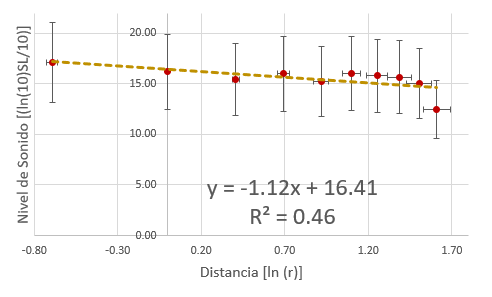
\includegraphics[width=1\textwidth]{grafica 700 Hz.PNG}
    \captionof{figure}{Gráfica del nivel de sonido vs la distancia para la frecuencia de $(700 \pm 1) Hz$}
    \label{fig}
\end{Figura}


\begin{Figura}
\centering
    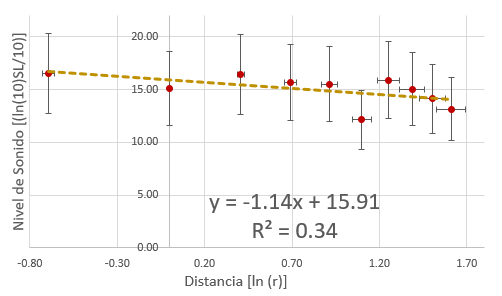
\includegraphics[width=1\textwidth]{grafica 800 Hz.PNG}
    \captionof{figure}{Gráfica del nivel de sonido vs la distancia para la frecuencia de $(800 \pm 1) Hz$}
    \label{fig}
\end{Figura}



\begin{Figura}
\centering
    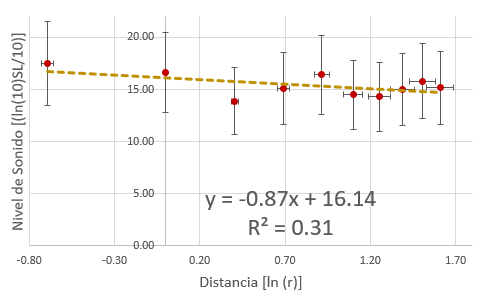
\includegraphics[width=1\textwidth]{grafica 900 Hz.PNG}
    \captionof{figure}{Gráfica del nivel de sonido vs la distancia para la frecuencia de $(900 \pm 1) Hz$}
    \label{fig}
\end{Figura}


\begin{Figura}
\centering
    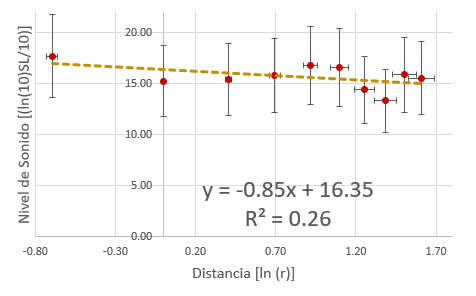
\includegraphics[width=1\textwidth]{grafica 1000 Hz.PNG}
    \captionof{figure}{Gráfica del nivel de sonido vs la distancia para la frecuencia de $(1000 \pm 1) Hz$}
    \label{fig}
\end{Figura}

Haciendo uso de la función en Excel 'ESTIMACION.LINEAL' se determinaron las incertidumbres de cada pendiente y se presentan en la siguiente tabla.


\begin{Figura}
\centering
    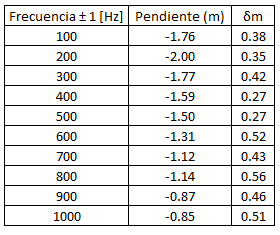
\includegraphics[width=0.8\textwidth]{pendientes.PNG}
    \captionof{figure}{Pendientes ajustadas con sus correspondientes incertidumbres para cada frecuencia}
    \label{fig}
\end{Figura}









\section*{Conclusiones}

Es difícil notar algún patrón de comportamiento en la gráfica presente en la figura 3 pero en la figura 4 se puede ver un comportamiento semejante para cada frecuencia solo que se van desplazando hacia arriba conforme aumenta la frecuencia hasta llegar a un punto donde parece detenerse. para las gráficas de las figuras 5-14 es notorio que para frecuencias por debajo de los $400 Hz$ la pendiente ajustada incluye en su intervalo dado por su incertidumbre  al valor esperado presente en la ecuación (4) sin embargo para frecuencias superiores esto ya no ocurre y además hay una mayor dispersión de los datos\footnote{Considero que esto fue debido al lugar donde se colocó el arreglo experimental y donde se realizo la practica ya que como se puede ver en la figura 1 y 2, existen varios muebles y paredes muy cerca de cada punto de medición, esto pudo causar alguna especie de eco que afecto las mediciones principalmente para las frecuencias más altas.}. 
  
\begin{thebibliography}{99}

\bibitem{1} Oda, Berta. Introducción al análisis gráfico de datos experimentales, las prensas de ciencias, 3ra ed. México, 2017.

\bibitem{2} ] Resnick, Robert; Halliday, David; Krane, Kenneth S. Física Vol. 2, Compañía Editorial Continental S.A. de C.V., 3ra ed. en español, México,
1999.



\end{thebibliography}

\section*{Apéndices}

\begin{Figura}
\centering
    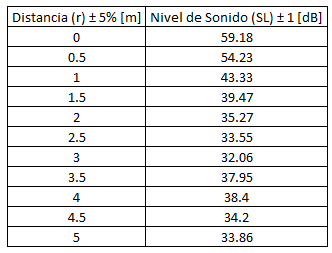
\includegraphics[width=0.8\textwidth]{tabla 100 Hz.PNG}
    \captionof{figure}{Tabla de nivel de sonido $SL$ registrado para cada distancia $r$ para la frecuencia de $(100 \pm 1) Hz$}
    \label{fig}
\end{Figura}


\begin{Figura}
\centering
    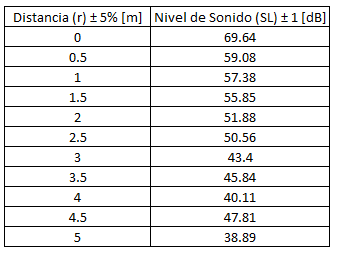
\includegraphics[width=0.8\textwidth]{tabla 200 Hz.PNG}
    \captionof{figure}{Tabla de nivel de sonido $SL$ registrado para cada distancia $r$ para la frecuencia de $(200 \pm 1) Hz$}
    \label{fig}
\end{Figura}


\begin{Figura}
\centering
    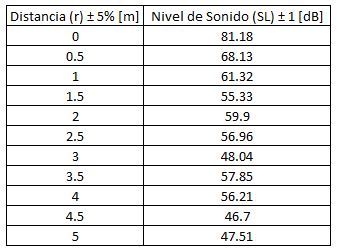
\includegraphics[width=0.8\textwidth]{tabla 300 Hz.PNG}
    \captionof{figure}{Tabla de nivel de sonido $SL$ registrado para cada distancia $r$ para la frecuencia de $(300 \pm 1) Hz$}
    \label{fig}
\end{Figura}


\begin{Figura}
\centering
    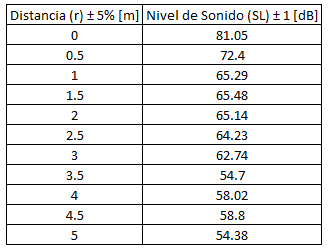
\includegraphics[width=0.8\textwidth]{tabla 400 Hz.PNG}
    \captionof{figure}{Tabla de nivel de sonido $SL$ registrado para cada distancia $r$ para la frecuencia de $(400 \pm 1) Hz$}
    \label{fig}
\end{Figura}


\begin{Figura}
\centering
    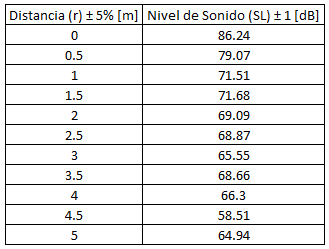
\includegraphics[width=0.8\textwidth]{tabla 500 Hz.PNG}
    \captionof{figure}{Tabla de nivel de sonido $SL$ registrado para cada distancia $r$ para la frecuencia de $(500 \pm 1) Hz$}
    \label{fig}
\end{Figura}


\begin{Figura}
\centering
    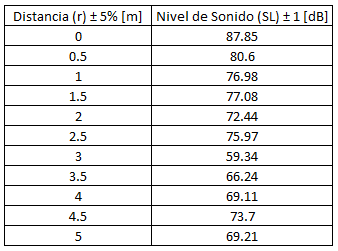
\includegraphics[width=0.8\textwidth]{tabla 600 Hz.PNG}
    \captionof{figure}{Tabla de nivel de sonido $SL$ registrado para cada distancia $r$ para la frecuencia de $(600 \pm 1) Hz$}
    \label{fig}
\end{Figura}


\begin{Figura}
\centering
    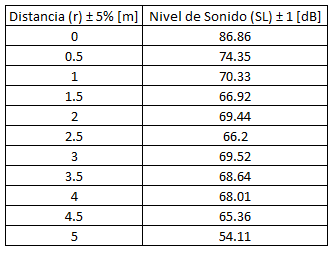
\includegraphics[width=0.8\textwidth]{tabla 700 Hz.PNG}
    \captionof{figure}{Tabla de nivel de sonido $SL$ registrado para cada distancia $r$ para la frecuencia de $(700 \pm 1) Hz$}
    \label{fig}
\end{Figura}


\begin{Figura}
\centering
    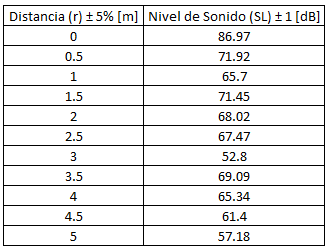
\includegraphics[width=0.8\textwidth]{tabla 800 Hz.PNG}
    \captionof{figure}{Tabla de nivel de sonido $SL$ registrado para cada distancia $r$ para la frecuencia de $(800 \pm 1) Hz$}
    \label{fig}
\end{Figura}


\begin{Figura}
\centering
    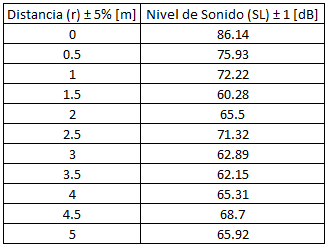
\includegraphics[width=0.8\textwidth]{tabla 900 Hz.PNG}
    \captionof{figure}{Tabla de nivel de sonido $SL$ registrado para cada distancia $r$ para la frecuencia de $(900 \pm 1) Hz$}
    \label{fig}
\end{Figura}


\begin{Figura}
\centering
    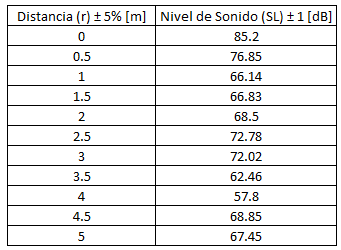
\includegraphics[width=0.8\textwidth]{tabla 1000 Hz.PNG}
    \captionof{figure}{Tabla de nivel de sonido $SL$ registrado para cada distancia $r$ para la frecuencia de $(1000 \pm 1) Hz$}
    \label{fig}
\end{Figura}


\end{multicols}
\end{document}